\chapter{Introduction}

Robotics and real life are worlds destined to meet. Today everyone has seen robots trying to behave like human beings. Many of them even look similar to a person and try to imitate the way we walk, talk or, ultimately, interact with the environment around us. 

Robots, Artificial Intelligence or other concepts such as Machine Learning have crept into our lives in just a few years. In fact, until recently, only a few visionaries like Marvin Minsky or Isaac Asimov used to speak of these concepts, and it was as part of science fiction novels. Nowadays, series like Black Mirror bring this technologies closer to the general public and make us reflect on how the future could be.

However, robots, and artificial intelligence in general, are still far from the vision that is told in the novels. They are not capable of understanding the environment around them, of learning or generalizing as we humans do. Companies and researchers are working on getting better generalization of the algorithms, but the truth is that, so far, Artificial Intelligence is only able to perform specific tasks for which they are programmed.

This project is one of those cases. The goal is to control a UR3 arm robot using Artificial Intelligence in order to pick disordered objects from a box and place them in a point of delivery. This task seems trivial, because we are used to see machines performing pick and place actions in industrial processes, but in fact, these kind of processes are normally just repeating the same action or the same rule over and over again. They are able to perform this tasks because they know apriori where these objects are or how they are placed, but they are not capable of generalizing the workflow. 

For instance, in Universal Robot free e-Learning course \cite{noauthor_formacion_nodate}, they expose the following example of an industry pick and place task. In
\autoref{fig:urconveyor} we can see how the robot is placing an object in a box located in a conveyor belt. The robot is using an infrared sensor to know that a box has arrived, and this box will always be in the same place because there is a stopper in the conveyor belt which doesn't allow the box to keep moving. On the other hand, the object is picked from the other conveyor belt using the same system to detect the arrival of a new object. The whole task is using a complex architecture, but the robot is performing the same chain of movements in a loop and the only intelligence that the robot has to have is waiting for the object and the box to come.

\begin{figure}
	\centering
	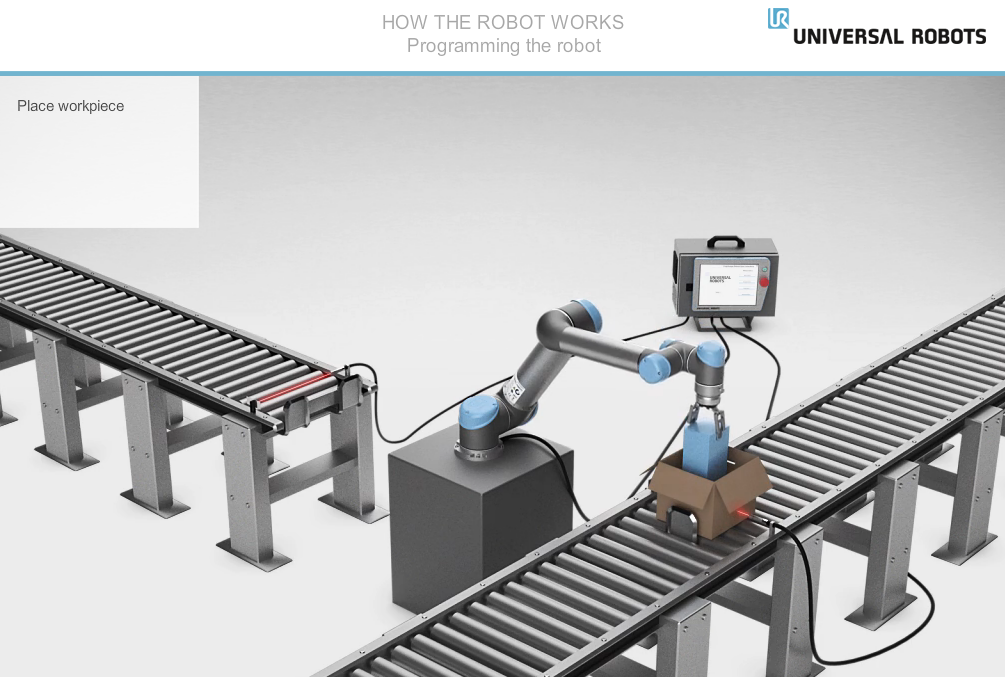
\includegraphics[width=0.85\linewidth]{Images/UR_conveyor}
	\caption[Pick and Place Task]{Universal Robots Pick and Place Task}
	\label{fig:urconveyor}
\end{figure}

To achieve generalization in this project, Reinforcement Learning (RL) together with Image Recognition techniques have been used. This algorithms give the robot the ability of calculating, for each time step, the optimal action to achieve the final goal of picking all the objects from the box and placing them in the objective point. To compute this action the robot needs to gather information about the environment such as its relative position over the box or how the pieces are distributed. This information together is called state, and the robot computes each action depending on it.

To perform this project, a distributed architecture with multiple nodes has been created. Each of them takes care of a different activity. For example, some nodes are used to control the robot, others to gather information about the current state, and others are used to train the Artificial Intelligence algorithm. This architecture has been created using ROS (Robot Operative System) and contributes to the project adding all the advantages of a microservices oriented architecture.

\section{Project Motivation}

The fourth industrial revolution is here, and it will change the way that goods are produced, raising efficiency by increasing the amount of automated processes. 
This will lead to a faster production and a reduction of errors, as machines have the ability to decide and act in fractions of seconds without making mistakes. Furthermore, machines can also be working 24 hours per day stopping just for maintenance checks, which would help to increase the productivity factor without increasing the expense in human resources.

We have been hearing about industry 4.0 since 2011, but the truth is that it is not a reality yet. We are just in the beginning, and it will take decades to perform such a big change in the industry. There are some factors to take in mind in order to analyse the evolution of the industry in the following years. The improvement on the telecommunications with the arrival of 5G networks, the moral dilemma of substituting workers for machines and the impact that this could have in the society or the improvement and implementation of AI technologies are just some of these factors. 

We have seen a lot of Artificial Intelligence algorithms applied to the industry, but the truth is that these technologies are not fully developed yet and just big companies can afford to use them in their supply chain. Besides, there are some task that are now performed by humans and cannot be done by machines due to its complexity or its importance in the whole production chain.

The motivation of this project is to contribute to the industry change providing an open source solution to a complex problem such as disordered pick and place task. This open source solution does not currently exist in the industry and would add value being a good starting point for bigger projects in the future.